\clearpage
\subsection{実習3-3 CdSセンサの電圧電流特性}
\begin{itemize}
	\item プログラムは上記の\ref{ex32-block}と同じものを利用し,$R_{0}$の値は10\,k\rm{$\Omega$}とした.
	\item 実行後,フロントパネルは\wfig{ex33-flont}のようになり,計測結果は\wtab{CDS}のようになった.
	\item 計測データを基に作成した電圧電流特性のグラフは\wfig{3-3}である.
\end{itemize}

 \begin{figure}[h]
  \centering
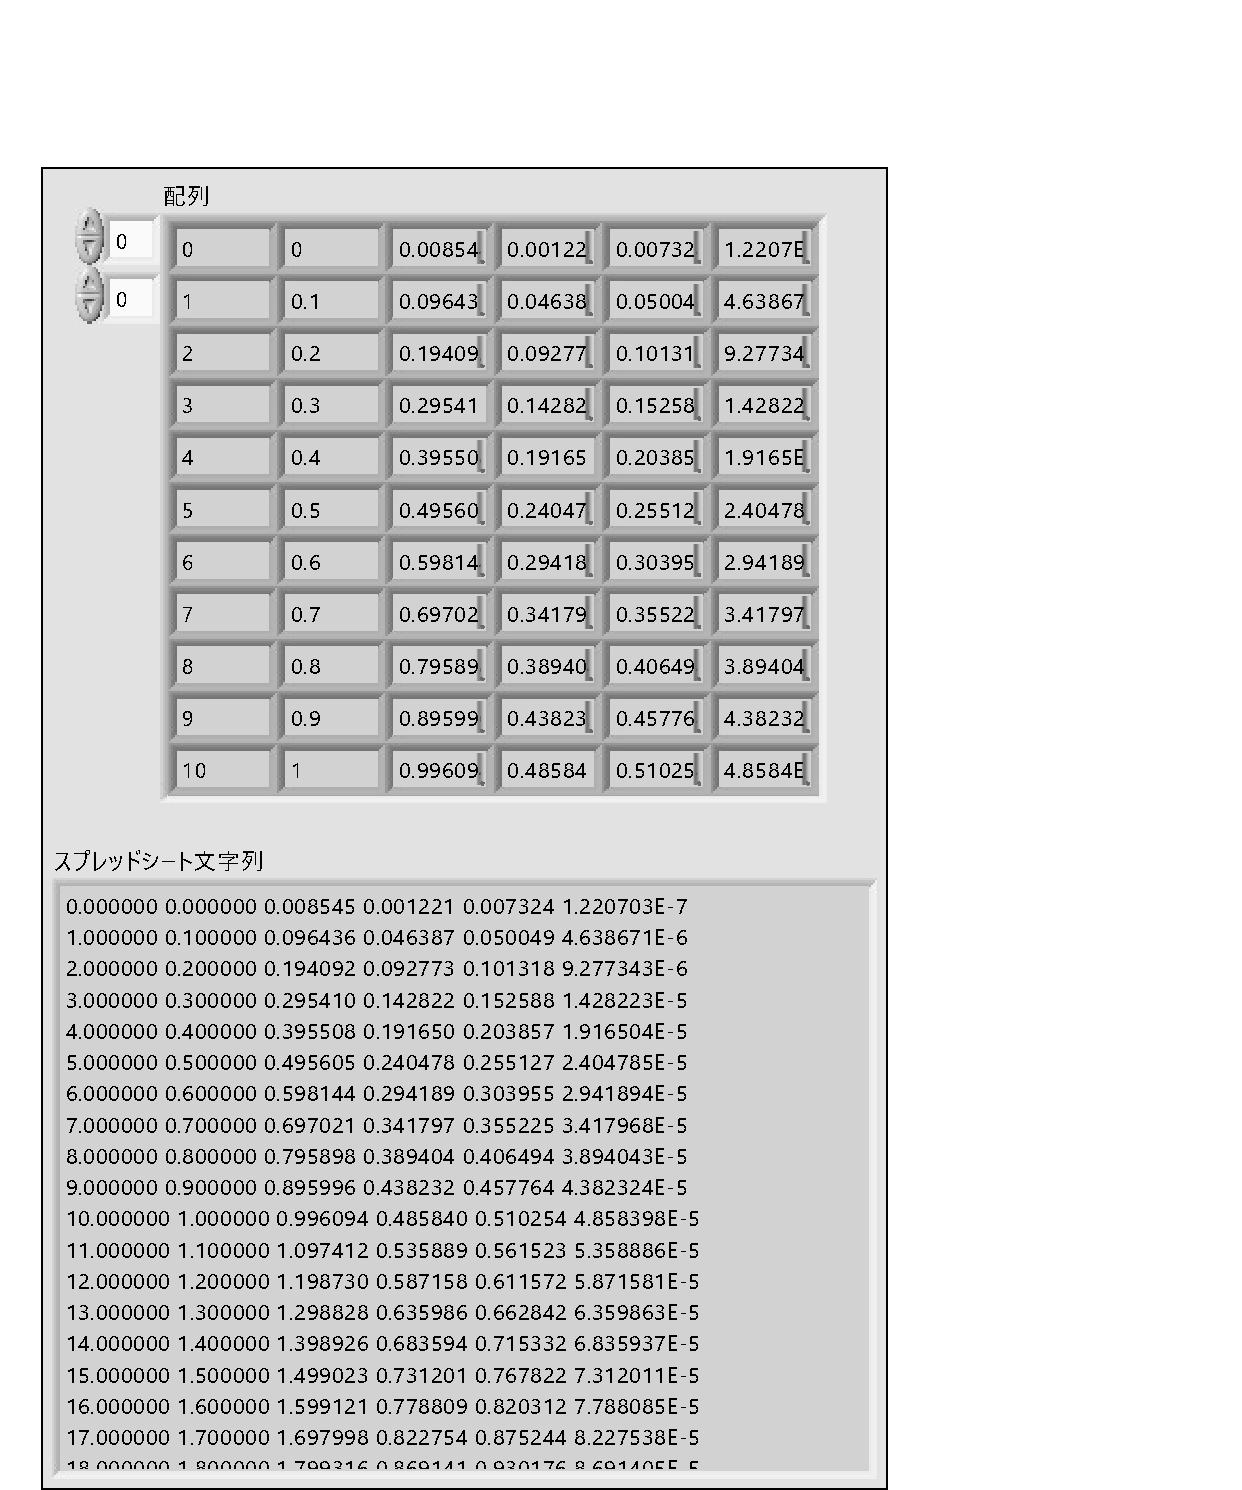
\includegraphics[scale=0.35]{./fig/ex33-flont.pdf}
\caption{CdSセンサの電圧電流特性測定時のフロントパネル}
\label{fig:ex33-flont}
\end{figure}

\begin{figure}[h]
\centering
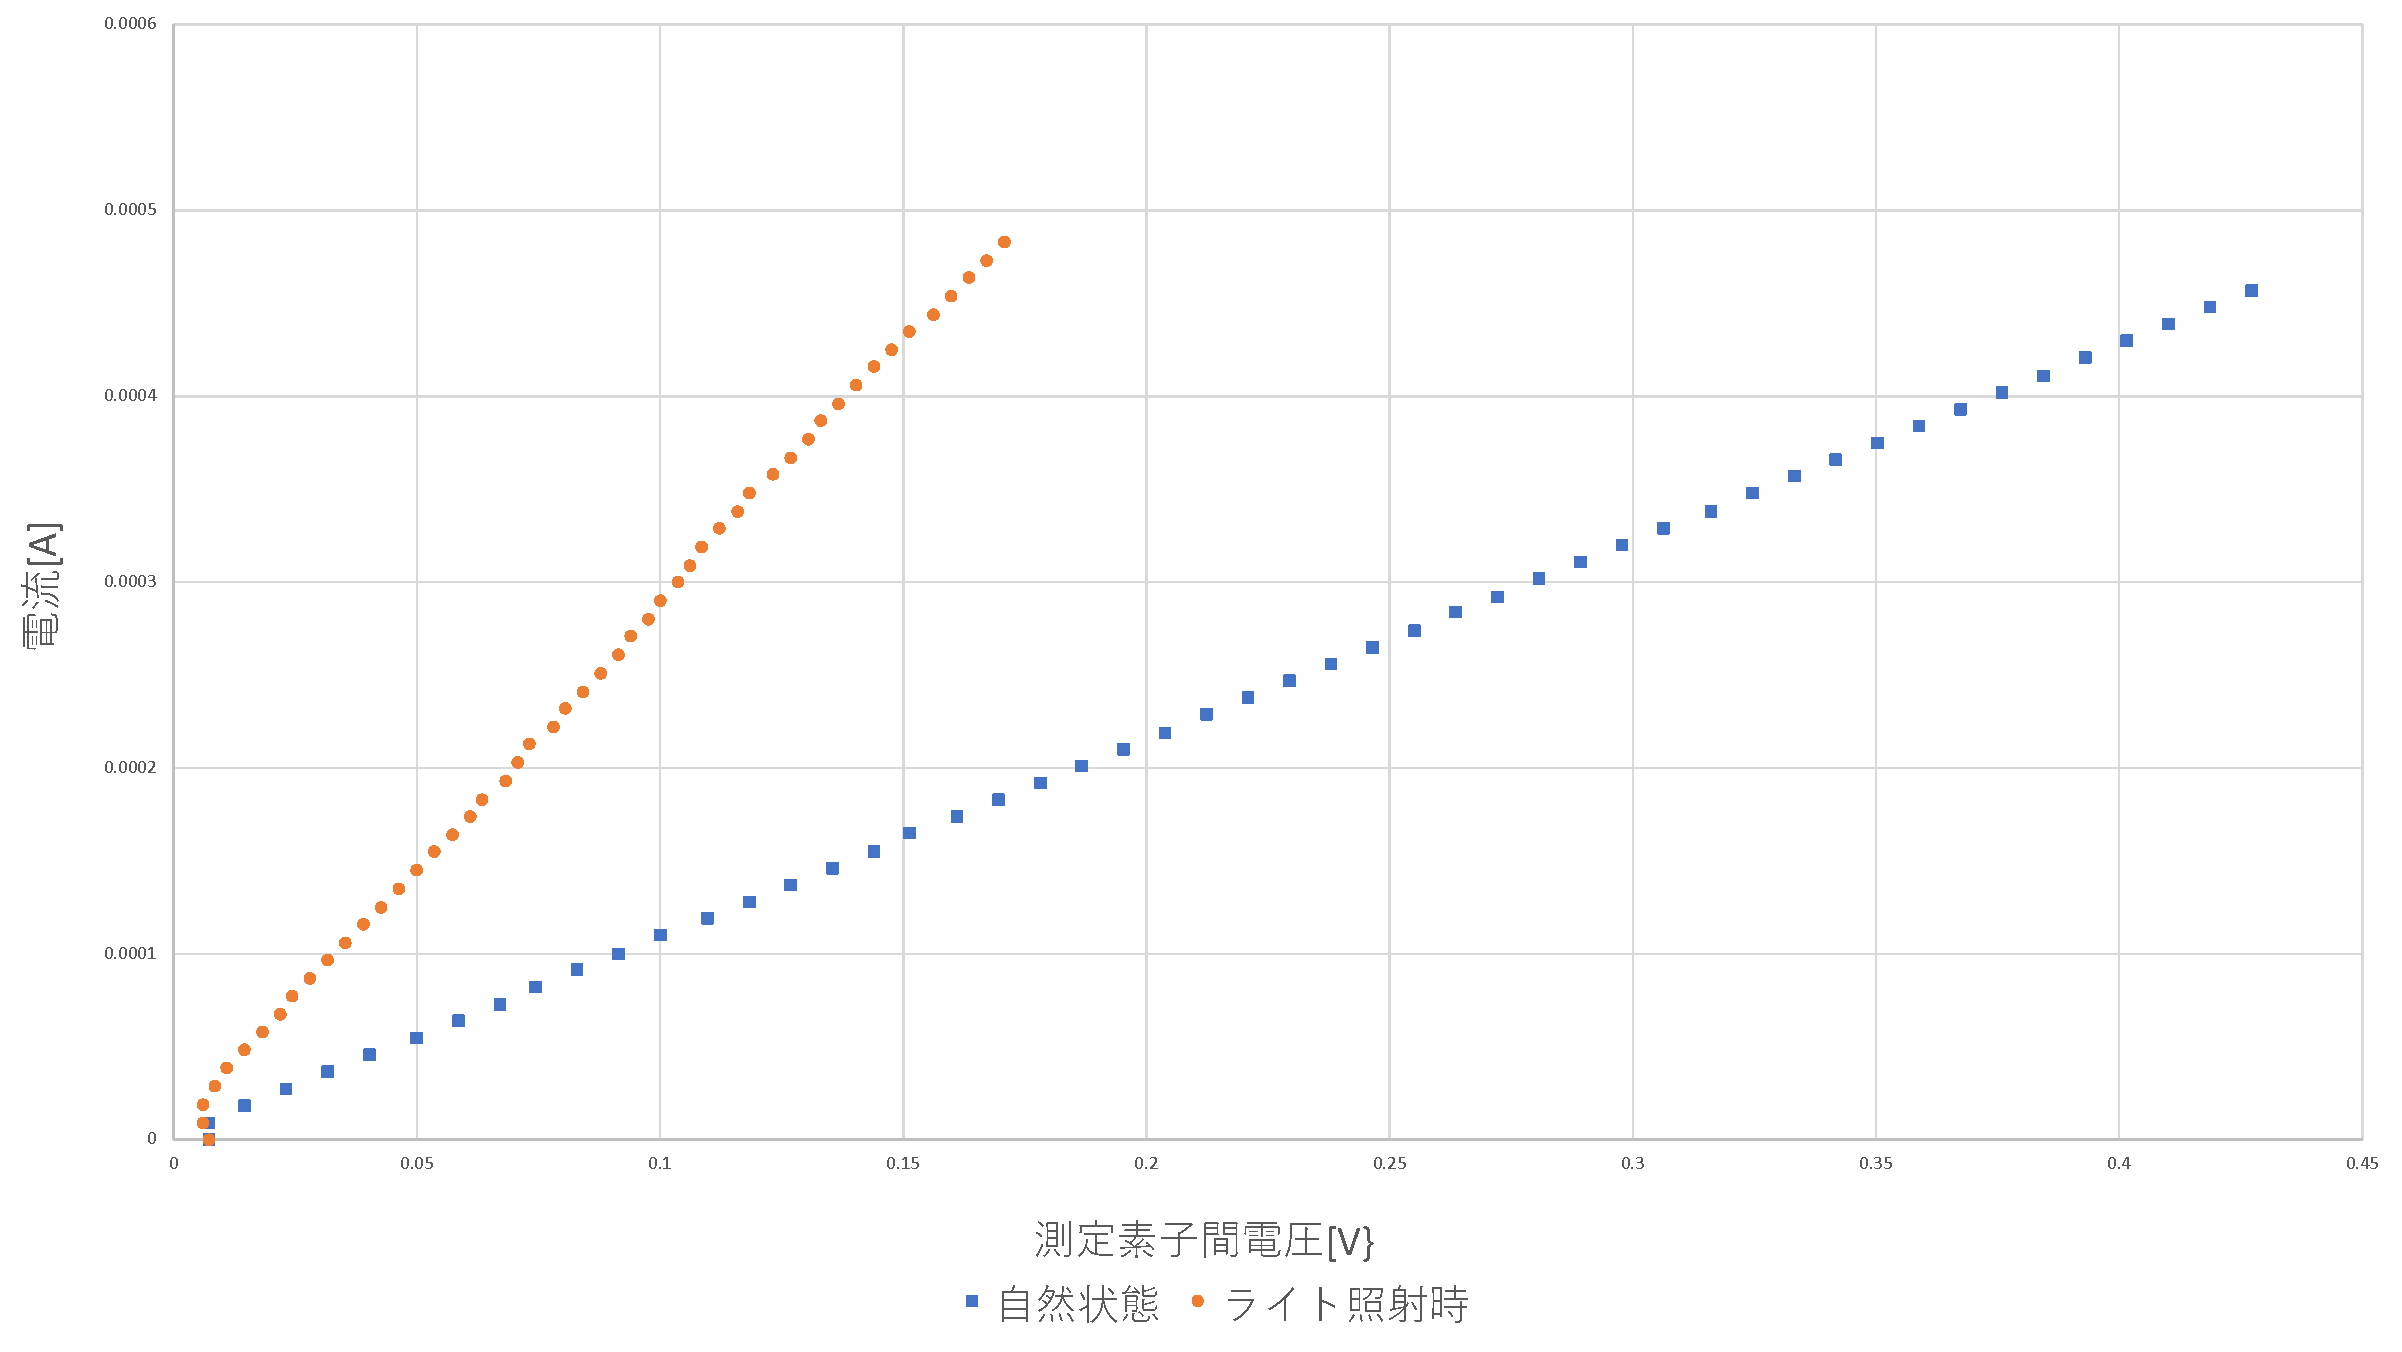
\includegraphics[scale=0.38]{./fig/3-3.pdf}
\caption{CdSセンサの電圧電流特性}
\label{fig:3-3}
\end{figure}

\begin{table}[h]
    \centering
    \caption{CdSセンサの諸特性値}
    \label{tab:CDS}
     \scalebox{0.7}{
    \begin{tabular}{ccccc}
    \hline
    カウンタ変数 & 自然状態での$V_{U}$[\rm{V}] & 自然状態での$I_{U}$[\rm{A}]  & ライト照射時の$V_{U}$[\rm{V}] &ライト照射時の$I_{U}$[\rm{V}]   \\
    \hline
0      & 0.007324 & 0        & 0.007324 & 0.0000000 \\
1      & 0.007324 & 0.000009 & 0.006104 & 0.0000092 \\
2      & 0.014648 & 0.000018 & 0.006104 & 0.0000189 \\
3      & 0.023193 & 0.000027 & 0.008545 & 0.0000289 \\
4      & 0.031738 & 0.000037 & 0.010986 & 0.0000387 \\
5      & 0.040283 & 0.000046 & 0.014648 & 0.0000483 \\
6      & 0.050049 & 0.000055 & 0.018311 & 0.0000580 \\
7      & 0.058594 & 0.000064 & 0.021973 & 0.0000675 \\
8      & 0.067139 & 0.000073 & 0.024414 & 0.0000774 \\
9      & 0.074463 & 0.000082 & 0.028076 & 0.0000868 \\
10     & 0.083008 & 0.000092 & 0.031738 & 0.0000966 \\
11     & 0.091553 & 0.0001   & 0.0354   & 0.0001060 \\
12     & 0.100098 & 0.00011  & 0.039062 & 0.0001160 \\
13     & 0.109863 & 0.000119 & 0.042725 & 0.0001250 \\
14     & 0.118408 & 0.000128 & 0.046387 & 0.0001350 \\
15     & 0.126953 & 0.000137 & 0.050049 & 0.0001450 \\
16     & 0.135498 & 0.000146 & 0.053711 & 0.0001550 \\
17     & 0.144043 & 0.000155 & 0.057373 & 0.0001640 \\
18     & 0.151367 & 0.000165 & 0.061035 & 0.0001740 \\
19     & 0.161133 & 0.000174 & 0.063477 & 0.0001830 \\
20     & 0.169678 & 0.000183 & 0.068359 & 0.0001930 \\
21     & 0.178223 & 0.000192 & 0.070801 & 0.0002030 \\
22     & 0.186768 & 0.000201 & 0.073242 & 0.0002130 \\
23     & 0.195312 & 0.00021  & 0.078125 & 0.0002220 \\
24     & 0.203857 & 0.000219 & 0.080566 & 0.0002320 \\
25     & 0.212402 & 0.000229 & 0.084229 & 0.0002410 \\
26     & 0.220947 & 0.000238 & 0.087891 & 0.0002510 \\
27     & 0.229492 & 0.000247 & 0.091553 & 0.0002610 \\
28     & 0.238037 & 0.000256 & 0.093994 & 0.0002710 \\
29     & 0.246582 & 0.000265 & 0.097656 & 0.0002800 \\
30     & 0.255127 & 0.000274 & 0.100098 & 0.0002900 \\
31     & 0.263672 & 0.000284 & 0.10376  & 0.0003000 \\
32     & 0.272217 & 0.000292 & 0.106201 & 0.0003090 \\
33     & 0.280762 & 0.000302 & 0.108643 & 0.0003190 \\
34     & 0.289307 & 0.000311 & 0.112305 & 0.0003290 \\
35     & 0.297852 & 0.00032  & 0.115967 & 0.0003380 \\
36     & 0.306396 & 0.000329 & 0.118408 & 0.0003480 \\
37     & 0.316162 & 0.000338 & 0.123291 & 0.0003580 \\
38     & 0.324707 & 0.000348 & 0.126953 & 0.0003670 \\
39     & 0.333252 & 0.000357 & 0.130615 & 0.0003770 \\
40     & 0.341797 & 0.000366 & 0.133057 & 0.0003870 \\
41     & 0.350342 & 0.000375 & 0.136719 & 0.0003960 \\
42     & 0.358887 & 0.000384 & 0.140381 & 0.0004060 \\
43     & 0.367432 & 0.000393 & 0.144043 & 0.0004160 \\
44     & 0.375977 & 0.000402 & 0.147705 & 0.0004250 \\
45     & 0.384521 & 0.000411 & 0.151367 & 0.0004350 \\
46     & 0.393066 & 0.000421 & 0.15625  & 0.0004440 \\
47     & 0.401611 & 0.00043  & 0.159912 & 0.0004540 \\
48     & 0.410156 & 0.000439 & 0.163574 & 0.0004640 \\
49     & 0.418701 & 0.000448 & 0.167236 & 0.0004730 \\
50     & 0.427246 & 0.000457 & 0.170898 & 0.0004830 \\
\hline
  \end{tabular}
  }
 \end{table}